\chapter{Material and Methods}\label{cap:studyOfTools}

% This chapter presents the technological tools used for the development of this work. Section~\ref{woodFurnitureIndustryTraceabilityReview} explores some concepts of ultrasonic sensors, specific characteristics of ultrasonic waves and the \gls{ToF} method for distance measurement. Then, in Section~\ref{embeddedSystem}, the definition, and a brief overview, of what an Embedded System is will be provided. Section~\ref{database} explores the definition and operation of a database and some basic database system architectures. At last, Section~\ref{webDevelopment} presents an overview of the operating mode of a web page and the programming languages which can be used for building it.


\section{Review of current traceability systems in the  industry}\label{woodFurnitureIndustryTraceabilityReview}

Atualmente, a rastreabilidade é empregada em diversos setores produtivos, apresentando uma ampla gama de aplicações. Entre elas, destacam-se a implementação de \acrfull{mcp} \cite{ZHONG2013}, controles de stock \cite{Anssens2011, Yue2011}, controle de produção \cite{Engelhardt2012}, prevenção de falsificações \cite{Rida2007}, entre outras possibilidades. A utilização de um sistema de rastreabilidade pode aprimorar significativamente a execução de tarefas em uma fábrica, permitindo não apenas um maior controle de inventário, mas também dos processos em si. Ao identificar pontos críticos na produção, é possível implementar ações para mitigar sua ocorrência e, consequentemente, tornar os processos mais eficientes \cite{Chua2012}.


Entretanto, é importante compreender o conceito de rastreabilidade. Segundo a norma ISO 9000:2015 \cite{iso_9000_2015}, rastreabilidade é definida como "ability to trace the history, application or location of that which is under consideration". Em outras palavras, no contexto de uma linha de produção, isso implica na habilidade de obter um histórico abrangente de informações pertinentes ao produto ou processo. Essas informações podem ser armazenadas de diversas maneiras, seja por meio de sistemas em papel, eletrônicos ou semi-eletrônicos.

Uma prática ainda prevalente, especialmente nas \acrfull{smes}\cite{ZHONG2013}, é a utilização de sistemas baseados em papel para a rastreabilidade dos produtos. No entanto, essa abordagem está sujeita a uma série de falhas decorrentes de erros humanos, dificuldades no gerenciamento das informações e, evidentemente, desafios consideráveis na implementação de modificações após o início da produção de um item \cite{Qu2012-hw}. Embora esse sistema seja consideravelmente ineficiente, ele continua a ser amplamente adotado \cite{ZHONG2013}.

Entretanto, um sistema híbrido pode ser adotado como uma abordagem que combina a utilização de sistemas tradicionais baseados em papel com a aplicação de tecnologias digitais, proporcionando um desempenho aprimorado no rastreamento de produtos, processos e registros de produção e estoque \cite{Qu2012-hw, ZHONG2013, Gilchrist2016}. Tal sistema é constituído por documentos impressos, planilhas, registros manuais, \acrshort{erp}, \acrshort{mes}, dentre outras soluções digitais.

Contudo, o sistema híbrido enfrenta desafios na obtenção de rastreabilidade em tempo real. Uma possibilidade para superar esses obstáculos, é necessário incorporar componentes de \acrfull{iot} e comunicação \acrshort{m2m}, possibilitando uma conexão em tempo real com o \acrshort{erp} ou permitindo a tomada de decisões sem a intervenção de um agente intermediário. A integração de tecnologias avançadas pode aprimorar significativamente a eficiência e a capacidade de adaptação do sistema híbrido, contribuindo para uma maior flexibilidade e precisão na rastreabilidade dos processos industriais \cite{Gilchrist2016}.

\subsection{Use of RFID for traceability}\label{RFIDtraceability}

A implementação de sensores \acrfull{rfid} é vastamente empregada na rastreabilidade de componentes na indústria, com aplicações em diversos setores \cite{ZHONG2013, Qu2012-hw, Anssens2011, Engelhardt2012, Rida2007}. O conceito inicial do RFID remonta ao artigo de Harry Stockman intitulado "Communication by Means of Reflected Power", publicado em 1948. A ideia demonstrou grande relevância na identificação de aeronaves pelo setor militar, especialmente devido aos avanços no desenvolvimento de radares ocorridos durante a Segunda Guerra Mundial \cite{Landt2005}. Essa inovação tecnológica permitiu melhorias significativas na eficiência e precisão da rastreabilidade, abrindo caminho para aplicações industriais e comerciais mais amplas no futuro.

No entanto, a implementação da tecnologia RFID requer uma infraestrutura específica, cuja viabilidade pode variar conforme o valor agregado proporcionado pelo seu uso. Para que o sistema RFID funcione adequadamente, são necessários alguns componentes fundamentais, tais como: uma antena, um transceptor, softwares middleware, um banco de dados e um transponder \cite{MCFARLANE2003365}. A figura \ref{fig:rfid} ilustra a configuração típica de um sistema RFID. 

\begin{figure}[h!]
    \centering
    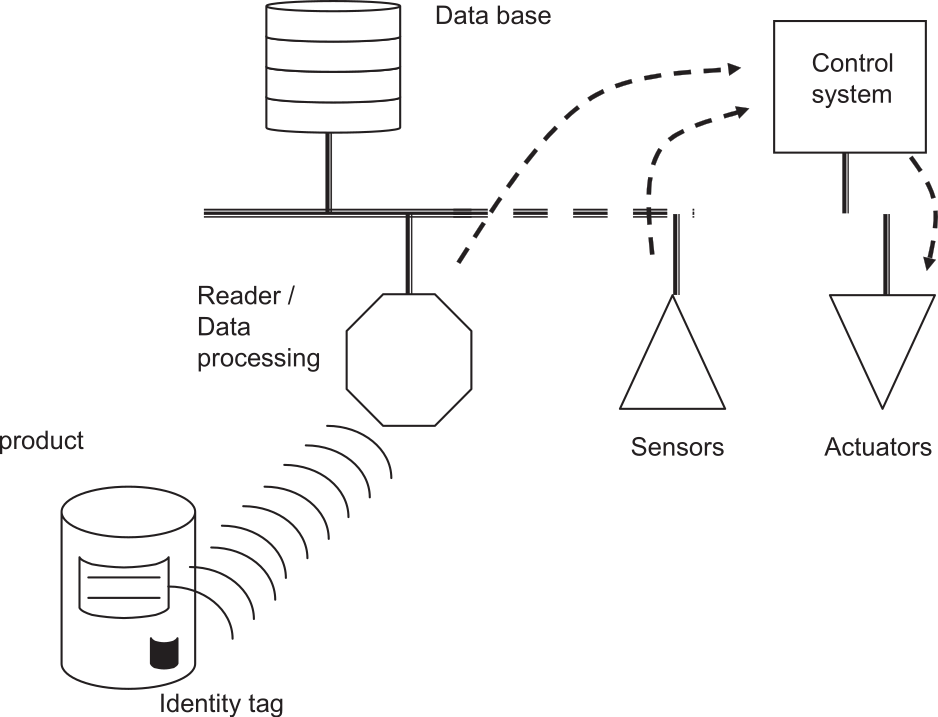
\includegraphics[width=.65\linewidth]{images/Development/chap3/g1126.png}
        \caption{Simple schematic of an Auto ID system. Source: \cite{MCFARLANE2003365}}

    \label{fig:rfid}
\end{figure}


Nesse contexto, a análise da viabilidade da adoção da tecnologia \acrshort{rfid} deve considerar os custos e benefícios associados à sua implementação. A infraestrutura necessária pode representar um investimento significativo, que deve ser justificado pelo retorno esperado em termos de eficiência operacional, redução de erros e otimização dos processos envolvidos. Portanto, a decisão de adotar a tecnologia \acrshort{rfid} deve ser embasada em uma avaliação criteriosa das necessidades específicas de cada aplicação e do valor que ela pode efetivamente agregar.

A seleção das tecnologias a serem utilizadas no sistema \acrshort{rfid} tem implicações diretas nos custos associados à sua implementação. Há três categorias de etiquetas \acrshort{rfid} disponíveis no mercado: passivas, ativas e passivas assistidas por bateria. Cada tipo apresenta características distintas, que influenciam tanto no desempenho quanto nos custos do sistema. Dentre as três opções, as etiquetas passivas são as mais econômicas. Essas etiquetas não possuem bateria interna e, consequentemente, são alimentadas pela energia transmitida pela antena do leitor. Apesar de serem mais acessíveis financeiramente, as etiquetas passivas possuem um alcance limitado e podem ser afetadas por interferências causadas por materiais metálicos e líquidos presentes no ambiente. Por outro lado, as etiquetas ativas e passivas assistidas por bateria, embora mais custosas, oferecem um alcance maior e maior resiliência a interferências \cite{Lee2012}. A escolha entre esses tipos de etiquetas deve levar em consideração as especificidades da aplicação, como a necessidade de maior alcance ou tolerância a interferências, bem como a disponibilidade de recursos financeiros para investimento na infraestrutura do sistema \acrshort{rfid}.


A análise de viabilidade para a implementação de um sistema de gerenciamento de estoque utilizando a tecnologia \acrshort{rfid} é uma tarefa intrincada, pois exige a ponderação de múltiplos fatores, como a previsibilidade do fluxo de estoque, os custos fixos e, principalmente, as tecnologias envolvidas no processo. Diversos estudos têm sido realizados para avaliar a viabilidade financeira do uso de \acrshort{rfid} em diferentes contextos.

\textcite{Yue2011}, por exemplo, conduziram uma simulação da viabilidade do uso de \acrshort{rfid} em uma cadeia de suprimentos do setor farmacêutico. Os autores concluíram que, utilizando o método do \acrfull{npv}, o empreendimento poderia não ser viável. Desse modo, sugeriram a utilização do método de \acrfull{rov} para uma análise mais precisa.

Em contrapartida, \textcite{Ustundag2007} realizaram um estudo de caso em uma transportadora de encomendas e constataram que o empreendimento é viável, embora o tempo de retorno varie conforme o tipo de etiqueta \acrshort{rfid} escolhida. Vale ressaltar que esse estudo de caso não apresenta detalhamento aprofundado.

Por fim, \textcite{Lee2012} apresentaram uma metodologia aprimorada para a avaliação financeira do investimento em sistemas de identificação por radiofrequência. Neste artigo, os autores introduzem um modelo matemático capaz de quantificar a viabilidade do empreendimento, levando em consideração o fluxo de estoque, os custos fixos e os modelos de estoque \acrfull{jit} ou \acrfull{eoq}. Neste modelo, os autores abordam três aspectos principais: 

\begin{enumerate}
  \item Investimento na eficiência do pedido;
  \item Investimento na eficiência do JIT;
  \item Decisões simultâneas de investimento em \acrfull{rfid}.
\end{enumerate}

O modelo matemático proposto por \textcite{Lee2012} é composto por quatro componentes de custo: custo do pedido durante um período de planejamento ($\frac{OD}{Q^*}$), fator de eficiência do processo atrelado à tecnologia \acrshort{rfid} (R), custo de manutenção do estoque ($ \frac{HQ^}{2} $), eficiência do \acrshort{jit} (I), custo de investimento para eficiência do pedido (K) e custo de investimento para eficiência \acrshort{jit} (V). A quantidade ótima de pedido, que minimiza o custo total, é representada pela equação \ref{eq:Lee}. 

A eficiência \acrshort{jit} aprimora-se conforme a taxa diária de entrega (d) se aproxima da taxa diária de consumo (c), como expresso na equação \ref{eq:Lee}. Neste modelo, os autores abordam três aspectos principais, sendo um deles a eficiência \acrshort{jit}, que é definida como o grau em que o intervalo de tempo entre o ponto de entrega e o tempo de consumo/produção é reduzido pelo investimento V.



\begin{equation} \label{eq:Lee}
\begin{split}
& TC = \frac{ORD}{Q^{}} + \frac{IHQ^}{2} + K + V \\
& Q^* = \sqrt{\frac{2ORD}{H I}} \\
& I = 1 - \frac{c}{d}, \quad 0 \leq I \leq 1.
\end{split}
\end{equation}

A equação \ref{eq:Lee} indica que um custo fixo de pedido mais elevado e um custo de manutenção de estoque mais alto contribuem para uma quantidade ótima de pedido maior. Este modelo matemático estabelece uma base sólida para a análise de investimentos em sistemas \acrshort{rfid}, possibilitando uma avaliação mais acurada da viabilidade financeira desses empreendimentos.

Ademais, com base na equação \ref{eq:Lee}, os autores conseguem deduzir alguns valores relevantes para analisar possíveis investimentos, como o valor ótimo de investimento para a tecnologia e o mínimo nível de demanda de fluxo de estoque necessário para que o empreendimento seja viável. Ou seja, matematicamente,  é possível analisar um caso opitimo que envolva condições restitivas.  Pra um caso em que os valores de investimento K e V são limitados por um valor B, têm se a condição de contorno: 
\begin{equation} \label{eq:Lee_boundary}
V + K  = B
\end{equation}

De acordo com \textcite{Lee2012}, ao aplicar o multiplicador de Lagrange $\xi$ \cite{François2004} no problema que minimiza o custo total (TC), obtém-se a seguinte função auxiliar:

\begin{equation} \label{eq:Lee_Lagrange}
\mathcal{L}(K, V , \xi) = \frac{ORD}{Q^{}} + \frac{IHQ^}{2} + K + V + \xi(K + V -B)
\end{equation}

Ao aplicar as derivadas parciais, é possível resolver esse problema pelo teorema de Lagrange \cite{François2004}, resultando nas seguintes equações para valores optimos:

\begin{equation} \label{eq:Lee_R}
R^* = \frac{Q^* + \beta ODN}{\beta O D}
\end{equation}

\begin{equation} \label{eq:Lee_I}
I^* = \frac{2 + \gamma H Q^* L}{\gamma H Q^*}
\end{equation}

\begin{equation} \label{eq:Lee_K}
K^* = \frac{\ln{\frac{R^* -N}{M -N}}}{-\beta}
\end{equation}

\begin{equation} \label{eq:Lee_V}
V^* = \frac{\ln{\frac{I^* -L}{U -L}}}{-\gamma}
\end{equation}

M representa a eficiência mais baixa adquirida na ausência de investimento em RFID, e N é a maior eficiência adquirida pelo investimento K.

Os autores realizaram uma simulação de um estudo de caso para ilustrar o modelo matemático proposto, utilizando os seguintes parâmetros:

\begin{itemize}
\item Custo fixo de pedido de \$10.000 por ciclo de pedido;
\item Custo anual de manutenção de inventário de \$1.000 por unidade;
\item Demanda anual de 120.000 unidades;
\item M 1,0;
\item N 0,3;
\item U 1,0;
\item L 0,2;
\item A 1,0;
\item E 0,5;
\item λ 0,000 01;
\item β 0,000 02.
\end{itemize}

Os resultados obtidos são apresentados nas figuras a seguir:

\begin{figure}[h!]
\centering
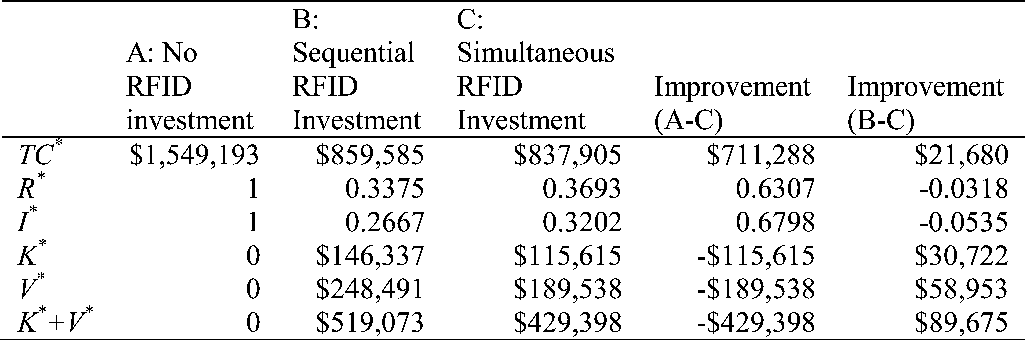
\includegraphics[width=.65\linewidth]{images/Development/chap3/table.png}
\caption{Cost saving by simultaneous RFID investment over sequential RFID investment (Table). Source: \cite{Lee2012}}
\label{fig:Lee_results_table}
\end{figure}

\begin{figure}[h!]
\centering
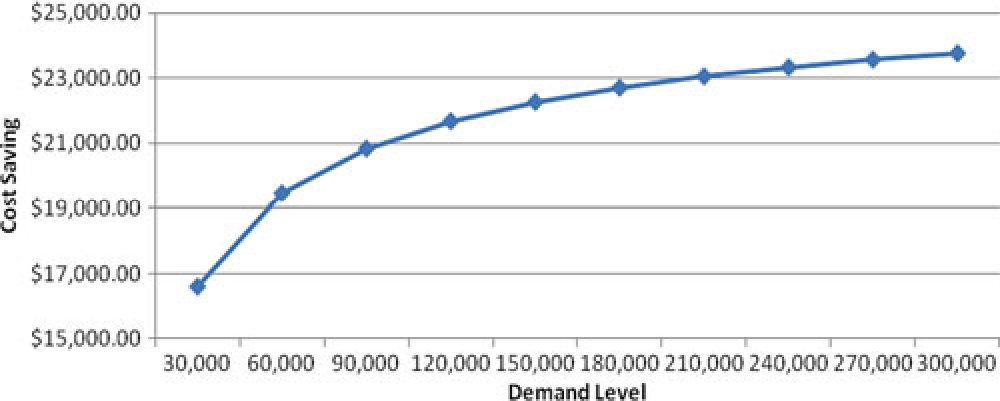
\includegraphics[width=.65\linewidth]{images/Development/chap3/chart.png}
\caption{Cost saving by simultaneous RFID investment over sequential RFID investment. Source: \cite{Lee2012}}
\label{fig:Lee_results}
\end{figure}

Em resumo, as contribuições dos autores \textcite{Lee2012} são bastante relevantes para uma modelagem mais precisa e fundamentada em métodos matemáticos. No entanto, para a obtenção de algumas constantes utilizadas no modelo matemático, o processo de análise do empreendimento pode ser bastante trabalhoso. Por outro lado, \textcite{Yue2011} e \textcite{Ustundag2007} utilizaram uma análise mais prática, que pode ser facilmente comparada caso empresas que desejam adotar o sistema de auto-ID por frequência de rádio tenham necessidades e estruturas semelhantes a esses estudos de caso.

No entanto, para o caso da empresa que é objeto do atual trabalho, o fluxo de estoque é bem menor em comparação aos três trabalhos analisados anteriormente, além de envolver produtos que podem não ter um valor tão alto agregado. Por essa razão, a adoção do sistema RFID pode não ser uma abordagem plausível.

\subsection{Use of QR Code for traceability}\label{QRtraceability}

O código QR, idealizado pela subsidiária da Toyota, Denso Wave, em 1994, foi estabelecido com o propósito de facilitar o rastreamento de componentes automobilísticos . A motivação por trás do desenvolvimento do código QR residia na limitação da capacidade de informação dos códigos de barras tradicionais, que comportam apenas 20 caracteres alfanuméricos. Essa inovação tecnológica provou sua eficiência ao proporcionar maior controle e exatidão no acompanhamento das peças empregadas na indústria automobilística \cite{Tiwari2016}.

Com o tempo, a aplicação do código QR se expandiu para diversos outros setores, consolidando-se como um instrumento valioso para aprimorar a rastreabilidade, a gestão de estoques, aplicações comerciais, emissão de ingressos para eventos, transações eletrônicas, e outras funcionalidades relevantes \cite{Tiwari2016}.

O funcionamento do sistema de código QR se baseia em dois componentes principais que atuam em conjunto para codificar e decodificar informações: o codificador de código QR e o decodificador. O codificador é responsável por processar os dados e gerar o QR Code, enquanto o decodificador extrai e interpreta os dados armazenados no código QR, veja a figura \ref{fig:qr}. A estrutura do QR Code é formada por módulos, que são os pontos pretos e brancos que compõem o código. Esses módulos são organizados em símbolos que variam da Versão 1 até a Versão 40, cada uma com uma configuração distinta de módulos, começando com a Versão 1, que contém 21 × 21 módulos, até a Versão 40, com 177 × 177 módulos \cite{iso_18004_2015}. Essa organização permite a codificação e decodificação eficiente de informações, garantindo a eficácia do QR Code como uma ferramenta de rastreabilidade e armazenamento de dados em diversos contextos e aplicações \cite{Tiwari2016}.


\begin{figure}[h!]
\centering
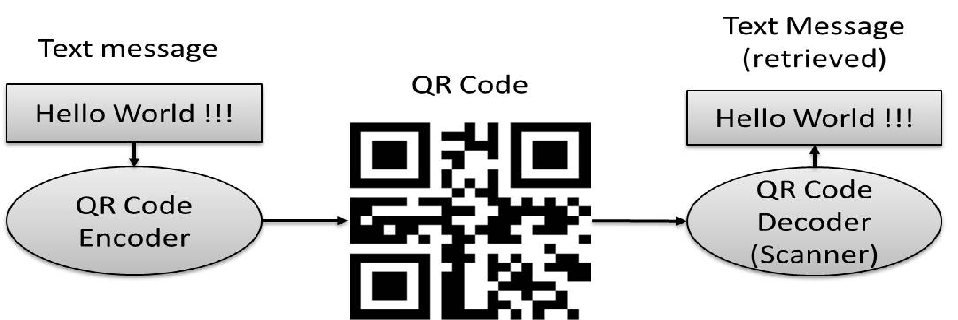
\includegraphics[width=.65\linewidth]{images/Development/chap3/QR.png}
\caption{Working (overview) of QR Code. Source: \cite{Tiwari2016}}
\label{fig:qr}
\end{figure}
Apesar das inúmeras vantagens do QR Code em relação ao código de barras, especialmente no que diz respeito à velocidade e capacidade de armazenamento de dados, o QR Code ainda possui limitações de capacidade. Cada versão do símbolo QR tem uma capacidade máxima de dados, que depende da quantidade de dados, do tipo de caractere e do nível de correção de erros \cite{Tiwari2016}. Em outras palavras, à medida que a quantidade de dados aumenta, são necessários mais módulos para compor o QR Code, resultando em um símbolo de QR Code maior, veja a tabela \ref{tab:qrcode-capacity}. Portanto, embora o QR ofereça benefícios significativos em termos de rastreabilidade e armazenamento de informações, é importante considerar suas limitações de capacidade ao selecionar a melhor solução para um determinado contexto ou aplicação.

\begin{table}[h]
\begin{tabular}{llllllll}
\hline
\multicolumn{8}{c}{DATA CAPACITY OF QR CODE VERSION 40 } \\
\cline{1-8}

Version             & Modules                  & ECC Level & Data Bits & Numeric & Alphanumeric & Binary & Kanji \\
\cline{1-8}


\multirow{4}{*}{40} & \multirow{4}{*}{177x177} & L         & 23,648    & 7,089   & 4,296        & 2,953 & 1,817 \\
                    &                          & M         & 18,672    & 5,596   & 3,391        & 2,331 & 1,435 \\
                    &                          & Q         & 13,328    & 3,993   & 2,42         & 1,663 & 1,024 \\
                    &                          & H         & 10,208    & 3,057   & 1,852        & 1,273 & 784 \\
\cline{1-8}
\end{tabular}
\caption{QR Code Capacity. Adapted from: \cite{Tiwari2016}}
\label{tab:qrcode-capacity}
\end{table}

Em conclusão, o código QR, concebido inicialmente com o objetivo de otimizar o rastreamento de componentes automobilísticos, tem experimentado uma evolução notável desde a sua criação, consolidando-se como uma ferramenta multifuncional e abrangente, aplicável em diversos setores. A capacidade de armazenar informações de maneira eficiente, aliada à facilidade de utilização por meio de dispositivos móveis e ao custo comparativamente inferior em relação a outras soluções, como a identificação por radiofrequência (RFID), confere ao código QR uma solução valiosa no aprimoramento da rastreabilidade e na gestão de dados em variados contextos. Entretanto, é crucial considerar as limitações inerentes à capacidade do código QR ao selecionar a alternativa mais adequada para atender às demandas específicas de rastreamento e armazenamento de informações. Nesse sentido, o código QR persiste como uma inovação tecnológica de relevância, capaz de proporcionar contribuições significativas à eficiência e eficácia dos processos de rastreabilidade, bem como ao armazenamento e compartilhamento de informações em ambientes distintos, dentro de suas limitações.


\subsection{Use of \acrshort{ai} in traceability}\label{ArtificialIntelligencetraceability}

Ao longo dos últimos anos, o crescimento exponencial do e-commerce tem impulsionado avanços significativos na gestão de armazenagem de mercadorias, devido ao aumento da escala e complexidade das operações envolvidas nesse âmbito. Atualmente, as empresas empregam uma ampla gama de tecnologias avançadas, tais como códigos QR, sistemas de visão de máquina, módulos de comunicação, microcomputadores, servidores e RFID, permitindo a integração de sistemas sofisticados que aplicam inteligência artificial na tomada de decisões estratégicas. Essa evolução tecnológica tem se mostrado crucial para aprimorar a gestão de armazenamento e otimizar a eficiência e eficácia das operações, atendendo às demandas crescentes e aos desafios impostos pelo comércio eletrônico em constante expansão \cite{Hristov2022}.


A aplicação da inteligência artificial em processos de rastreabilidade transcende a tomada de decisões no contexto industrial. Por exemplo, os autores \textcite{Hristov2022} empregaram \acrfull{cnn} na detecção de objetos, possibilitando que robôs identificassem itens em um centro de armazenamento e, consequentemente, agilizassem a tomada de decisões na realização de suas tarefas. Essa abordagem inovadora demonstra o potencial da inteligência artificial para aprimorar a eficiência e a precisão dos processos de rastreabilidade, além de permitir a rastreabilidade de inventário, contribuindo para uma maior adaptabilidade e dinamismo nas operações de armazenamento e movimentação de mercadorias.


O emprego de códigos de barras e RFID é uma prática amplamente adotada no rastreamento de produtos, tanto na produção quanto no estoque. Contudo, esses métodos apresentam algumas limitações. O uso de códigos de barras, por exemplo, possui uma capacidade restrita de armazenamento de informações e pode ser facilmente danificado, o que impossibilita a leitura. Adicionalmente, o emprego de RFID também enfrenta a problemática de possíveis danos, além dos custos elevados associados à infraestrutura necessária para seu funcionamento \cite{Pihir2011}. Os autores \textcite{Elisabeth2011} também mencionam as dificuldades do uso de RFID para certos tipos de materiais que podem interferir na leitura das ondas de rádio, o que pode demandar etiquetas mais robustas e aumentar ainda mais os custos envolvidos.


Em contraste com os métodos tradicionais de rastreamento de itens, os autores \textcite{Patel2020} propõem uma abordagem inovadora utilizando \acrshort{cnn}, especificamente com a arquitetura ResNet-50. Nessa metodologia, empregaram técnicas de transferência de aprendizado para viabilizar a adaptação ágil do modelo de dados em cenários com quantidade limitada de imagens para treinamento. Consequentemente, alcançaram uma taxa de rastreamento de imagem de 4 \acrfull{fps}, considerando as configurações de software e hardware adotadas, possibilitando a rastreabilidade de objetos em tempo real. Os autores também enfatizam o potencial desta abordagem na automação de processos com robôs que utilizam visão computacional, figura \ref{fig:robots}, o que pode minimizar a necessidade de intervenção humana no gerenciamento dos componentes armazenados e, assim, reduzir erros.

\begin{figure}[h!]
\centering
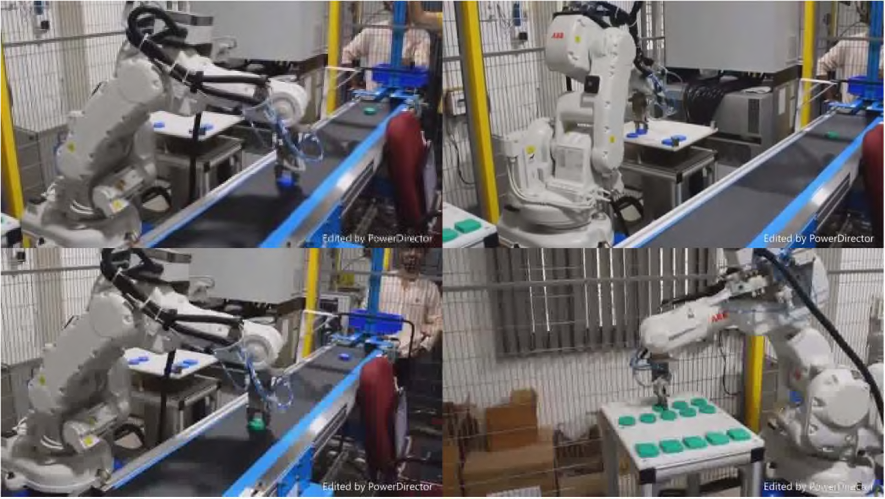
\includegraphics[width=.5\linewidth]{images/Development/chap3/robots.png}
\caption{A robot identifying the incoming objects and
selecting the correct action to perform. Source: \cite{Tiwari2016}.}
\label{fig:robots}
\end{figure}

Outro aspecto importante a ser considerado é a possibilidade de personalização das \acrshort{cnn} para atender às necessidades específicas de diferentes indústrias e setores. Através da utilização de arquiteturas e algoritmos apropriados, é possível desenvolver soluções de rastreamento adaptadas às particularidades de cada cenário, otimizando a eficiência e a eficácia das operações.


\section{Digital Image Processing}\label{subsec:imageProcessing}

O processamento digital de imagens é um campo que aborda a manipulação, análise e interpretação de imagens digitais, que são funções bidimensionais discretas, $f(x_i, y_i)$, compostas por elementos chamados pixeis. Essa disciplina engloba um amplo espectro de aplicações e se relaciona com áreas como análise de imagens e visão computacional. O processamento digital de imagens pode ser dividido em processos de baixo, médio e alto nível. Processos de baixo nível envolvem pré-processamento e aprimoramento de imagens, enquanto processos de médio nível lidam com segmentação, descrição e classificação de objetos. Já processos de alto nível buscam dar sentido a conjuntos de objetos reconhecidos e realizar funções cognitivas associadas à visão. O processamento digital de imagens abrange processos que trabalham com entradas e saídas de imagens e também processos que extraem atributos de imagens, incluindo o reconhecimento de objetos individuais, sendo aplicado com sucesso em diversas áreas de valor social e econômico  \cite{gonzalez_rafael_c_digital_2018}.


Neste campo multidisciplinar, uma ampla gama de técnicas e algoritmos é empregada para otimizar a qualidade das imagens, realçar características de interesse e facilitar a extração de informações valiosas. Tais abordagens podem ser aplicadas em diversos contextos, abrangendo desde a melhoria da qualidade de imagens obtidas por dispositivos fotográficos digitais até a análise de dados em imagens para aplicações específicas \cite{ekstrom2012}. 

Contudo, conforme relatado por \textcite{mcandrew2004introduction}, o processamento de imagem aborda dois aspectos distintos e fundamentais:
\begin{enumerate}
\item Aprimorar a informação pictórica para interpretação humana.
\item Tornar a imagem mais adequada para percepção autônoma de máquinas.
\end{enumerate}
O primeiro aspecto se refere ao aprimoramento da informação pictórica de uma imagem visando à interpretação humana, o que envolve melhorar a aparência visual da imagem. Já o segundo aspecto visa tornar a imagem mais adequada para a percepção autônoma de máquinas, o que implica em simplificar e organizar a imagem de maneira eficiente. Essas duas condições requerem procedimentos distintos e especializados, sendo que um procedimento que satisfaça uma condição pode não necessariamente satisfazer a outra. Como pode ser observado na figura \ref{fig:imageProcessingExample}, apesar de a imagem processada apresentar maior significância para uma análise de contornos, ela pode não ter um aspecto atrativo para o olho humano.

\begin{figure}[h!]
\begin{minipage}{0.45\linewidth}
\centering
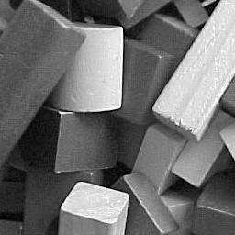
\includegraphics[scale=.65]{images/Development/chap3/woods_original.png}\\\\
(a) The original image
\end{minipage} \hspace{0.025\linewidth}
\begin{minipage}{0.45\linewidth}
\centering
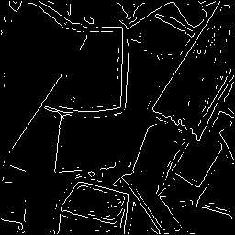
\includegraphics[scale=.65]{images/Development/chap3/woods_processed.png}\\\\
(b)  Its edge image
\end{minipage}
\caption{Example of image processing where the author tries to find the edges of the objects in the original image (a) and gets the image as a result (b). Source \cite{mcandrew2004introduction}. }
\label{fig:imageProcessingExample}
\end{figure}


Adicionalmente, o processamento de imagens desempenha um papel fundamental no desenvolvimento de sistemas de visão computacional e aprendizado de máquina, permitindo que dispositivos eletrônicos e máquinas interpretem e compreendam informações visuais de maneira análoga à percepção humana. Essa capacidade de processar e analisar imagens é imprescindível para a concepção de soluções inovadoras em áreas como robótica, automação industrial, segurança e vigilância, reconhecimento facial, entre outras.

Em síntese, o processamento de imagens constitui uma área de estudo abrangente e multidisciplinar, que engloba conhecimentos de ciência da computação e engenharia, visando aprimorar a qualidade das imagens digitais e extrair informações relevantes para uma vasta gama de aplicações. Através da aplicação de técnicas avançadas e algoritmos especializados, o processamento de imagens contribui significativamente para o progresso da visão computacional e aprendizado de máquina, impulsionando a inovação e o desenvolvimento tecnológico em diversos setores.


\subsection{Gaussiang Filtering}

A aplicação de um filtro em uma imagem implica na realização de uma operação de convolução. No contexto contínuo e com uma única variável no domínio, essa operação pode ser representada pela equação \ref{eq:convolution} \cite{spiegel_schaums_1974}. No entanto, ao trabalhar com imagens digitais, é comum empregar uma adaptação dessa equação para meios discretos em um domínio bidimensional, que faz uso de uma matriz-base, denominada kernel, conforme ilustrado na equação \ref{eq:convolution-discreet} \cite{gonzalez_rafael_c_digital_2018}. O kernel é utilizado para atribuir pesos aos pontos vizinhos de um ponto específico da imagem, modificando seus valores e resultando em uma imagem com pixeis alterados. Durante a convolução, o kernel é aplicado a cada ponto da imagem, multiplicando seus pesos pelos valores dos pixeis adjacentes, veja a imagem \ref{fig:kernel-convolution}. 

\begin{equation}
(f * g)(t) = \int_{-\infty}^{\infty} f(\tau) \cdot g(t-\tau) d\tau
\label{eq:convolution}
\end{equation}

\begin{equation}
(f * w)(x_i, y_i) = \sum_{s=-a}^{a} \sum_{t=-b}^{b} f(x_i +s, y_i +t) \cdot w(s, t) \quad \forall i \in \mathbb{N}
\label{eq:convolution-discreet}
\end{equation}\\


\begin{figure}[h!]
\centering
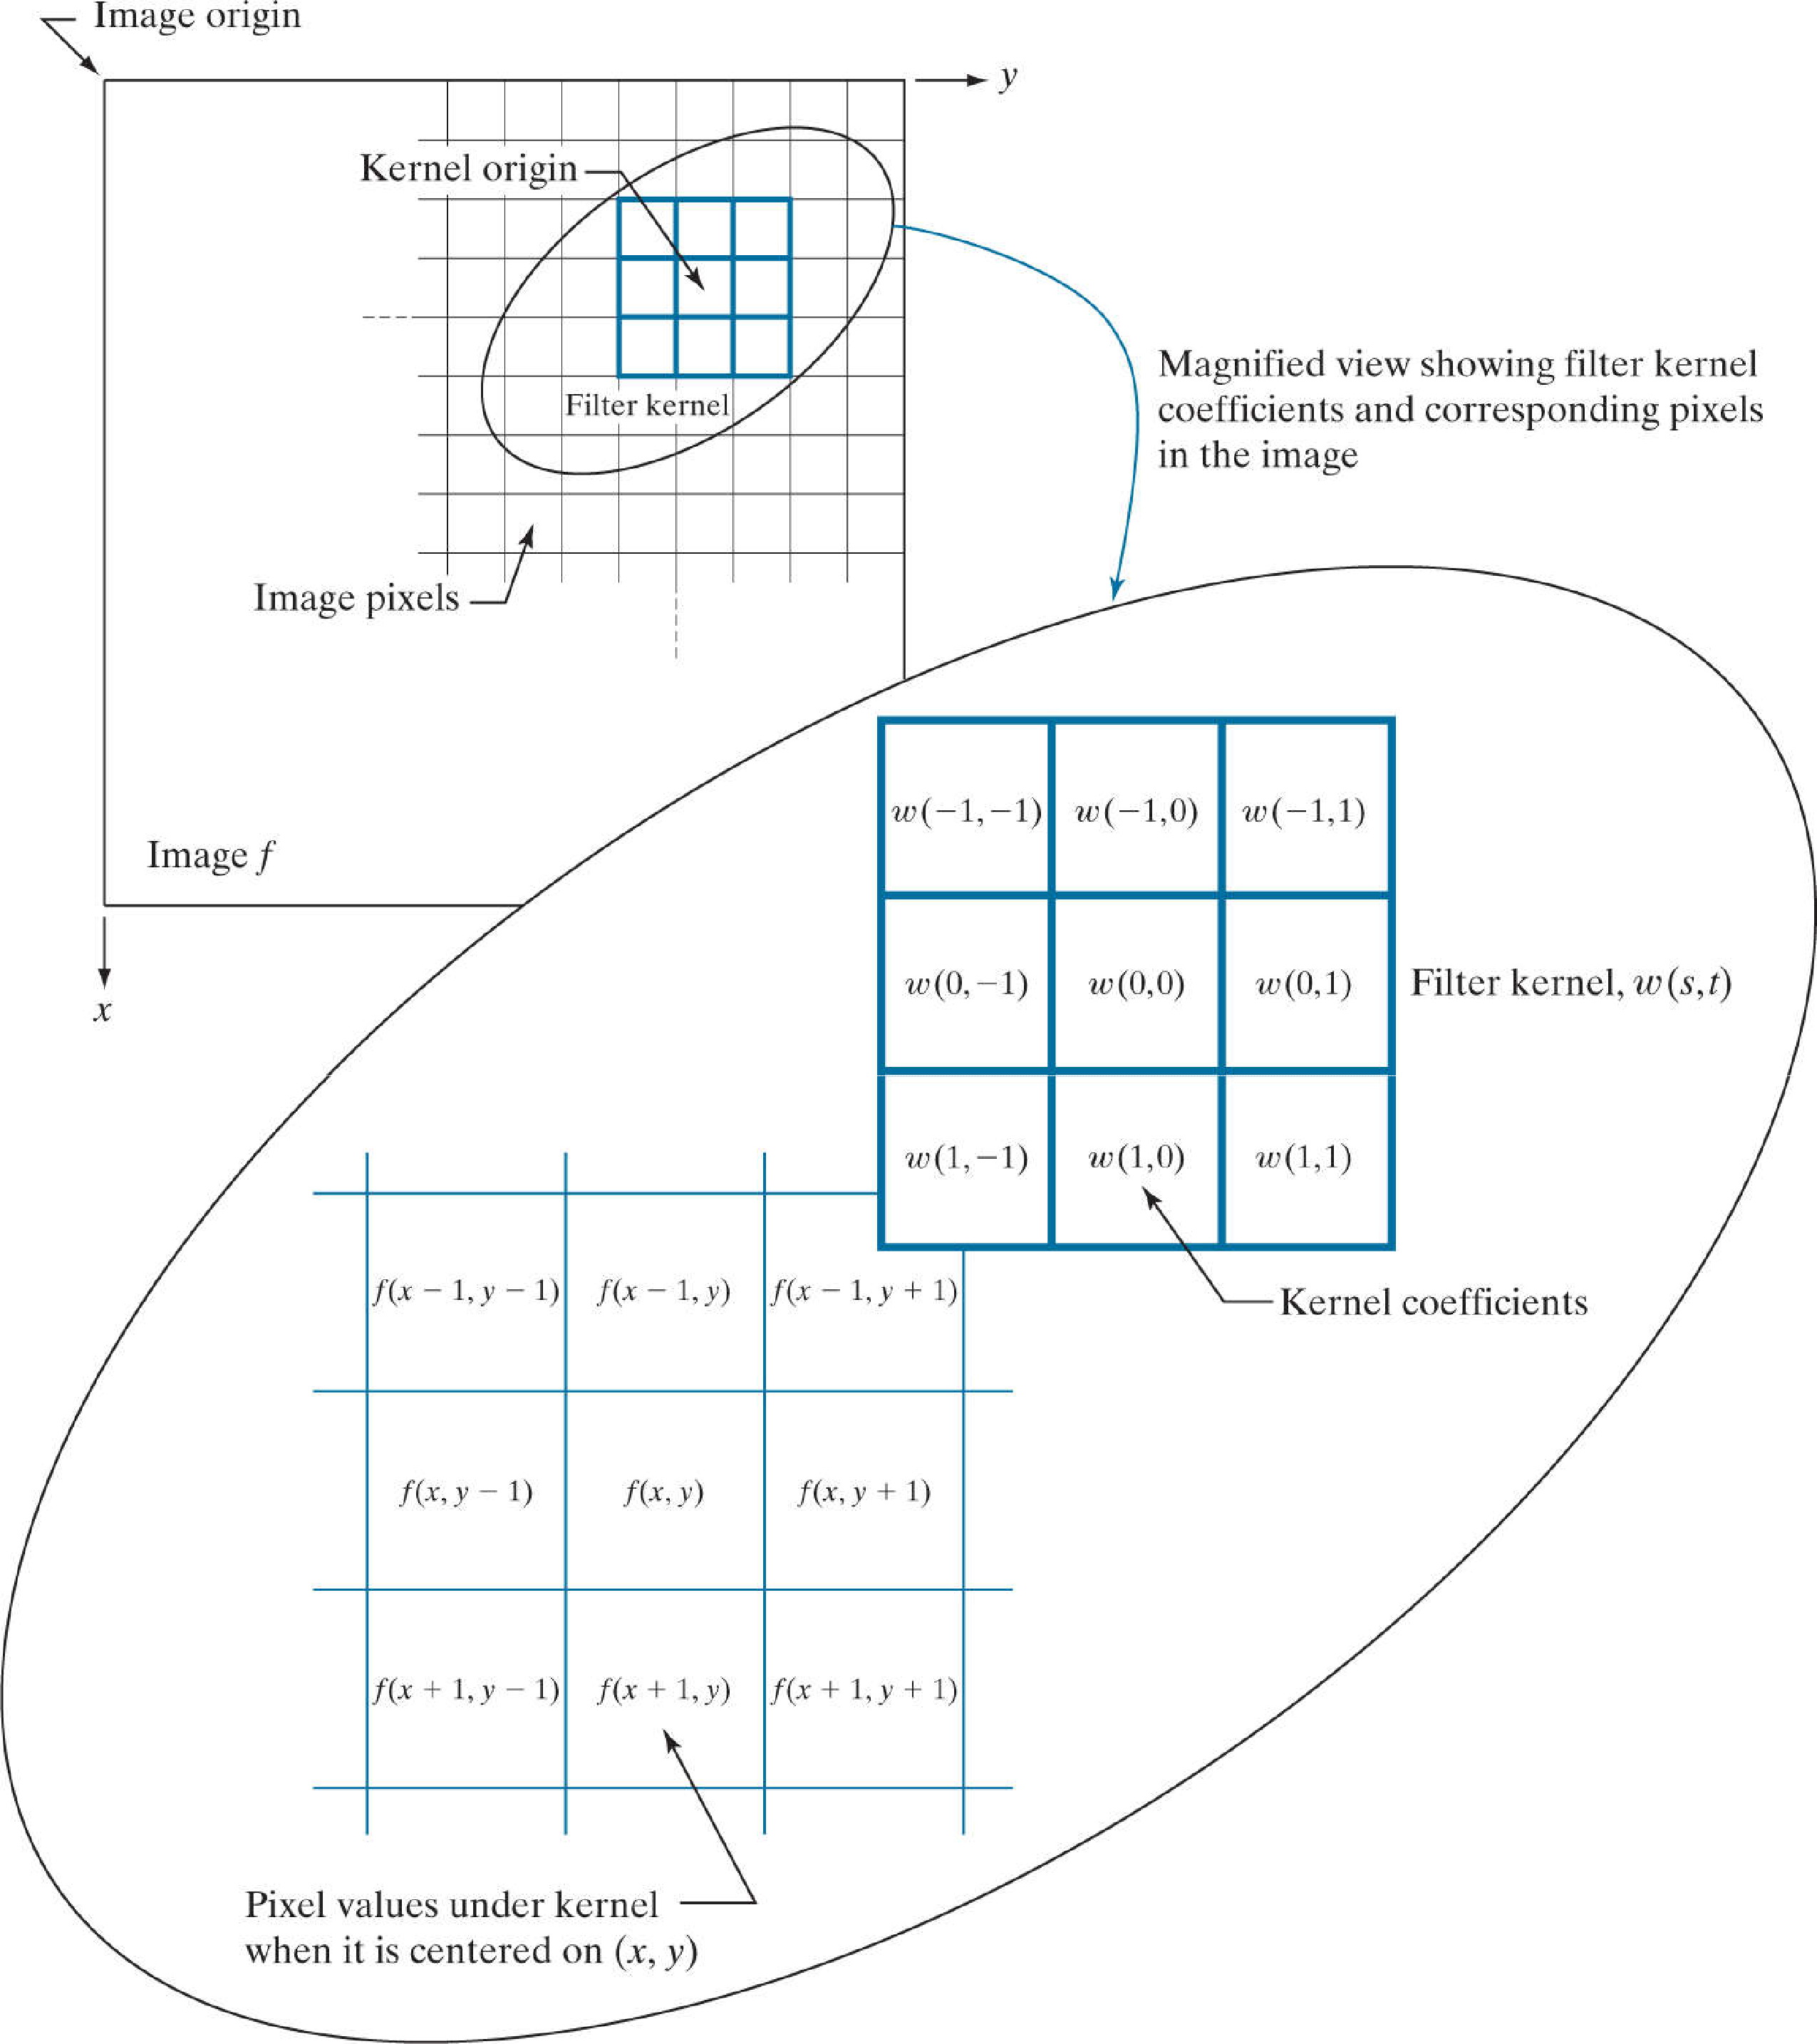
\includegraphics[width=.65\linewidth]{images/Development/chap3/kernel.png}
\caption{Kernel convolution representation on a digital image. Source: \cite{gonzalez_rafael_c_digital_2018}.}
\label{fig:kernel-convolution}
\end{figure}


Os filtros espaciais lineares são amplamente utilizados e empregam um kernel que realiza a soma de produtos entre a imagem original e o próprio kernel, figura \ref{fig:kernel-transformation}. O tamanho do kernel define a vizinhança de operação, enquanto seus coeficientes determinam a natureza do filtro. Vale ressaltar que diferentes kernels podem ser aplicados para distintas finalidades, como aprimorar a nitidez, realçar detalhes ou detectar bordas \cite{gonzalez_rafael_c_digital_2018}.

\begin{figure}[h!]
\centering
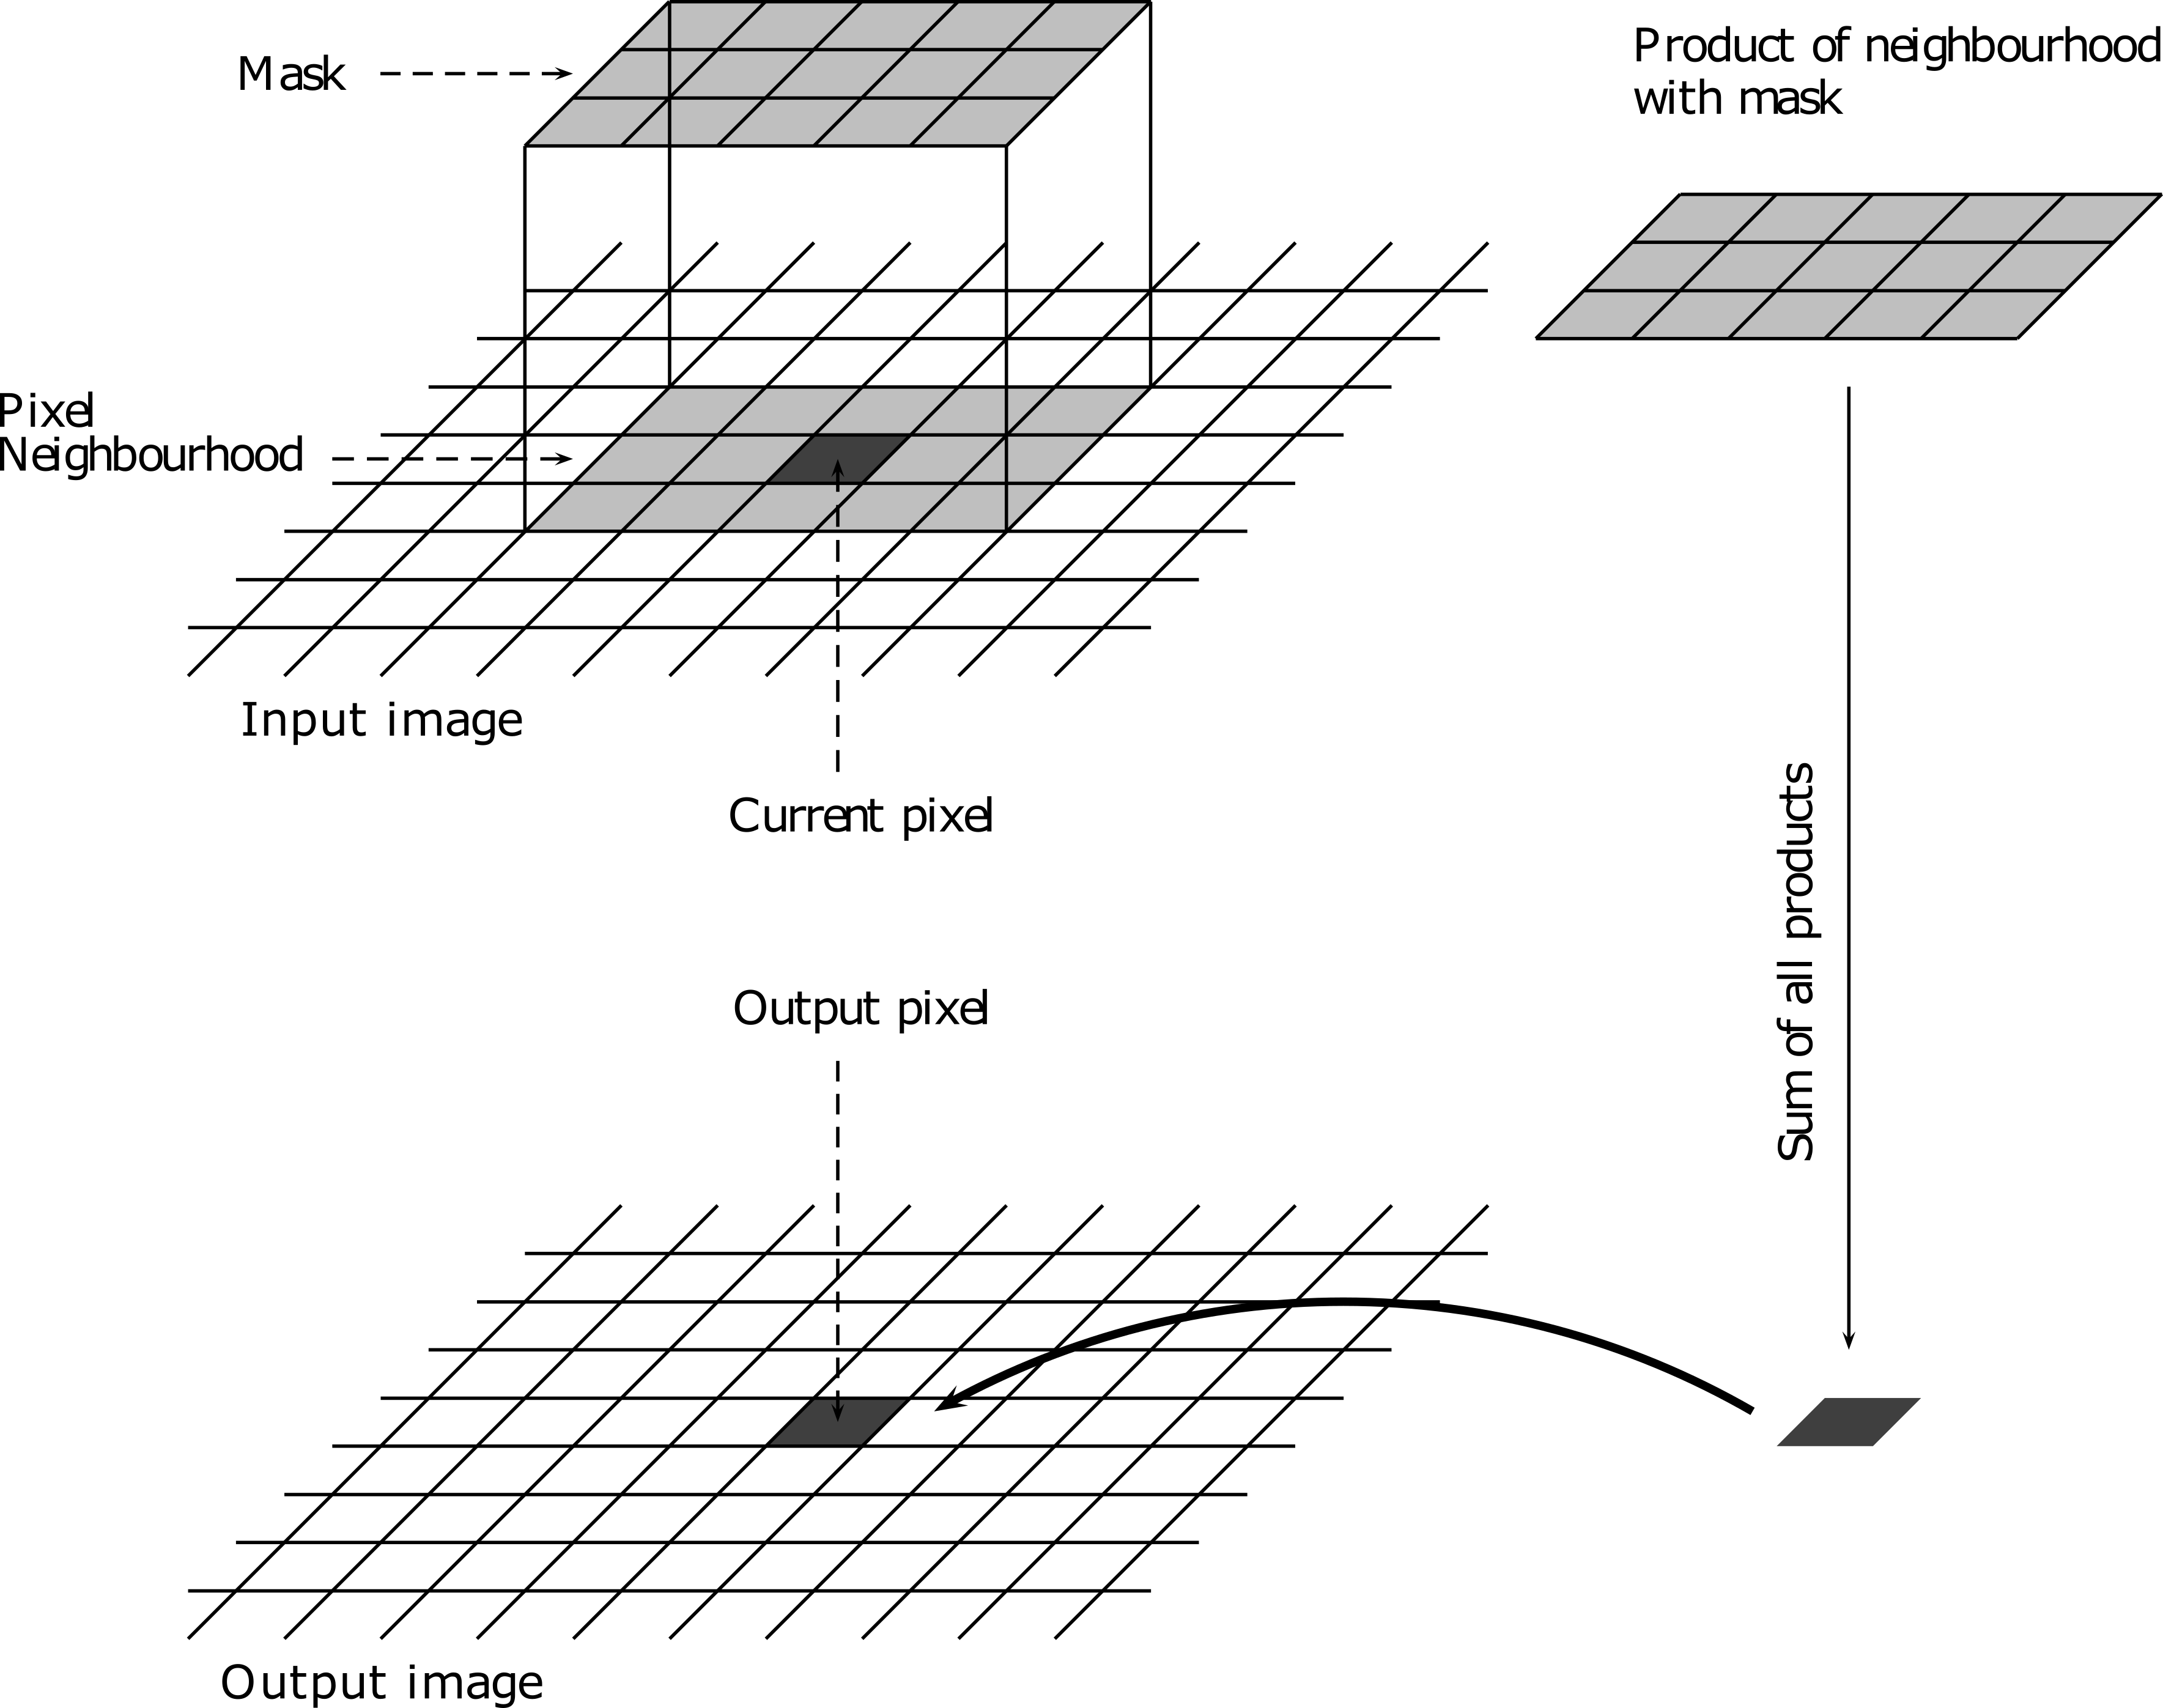
\includegraphics[width=.65\linewidth]{images/Development/chap3/transformation.png}
\caption{Performing spatial filtering. Source: \cite{mcandrew2004introduction}.}
\label{fig:kernel-transformation}
\end{figure}

Ademais, diversos tipos de filtros podem ser combinados para alcançar resultados mais sofisticados. Por exemplo, filtros de suavização e de realce podem ser utilizados em conjunto para produzir imagens mais nítidas e detalhadas. O processo de aplicação de filtros pode ser repetido várias vezes até obter o resultado desejado; contudo, é fundamental considerar que o uso excessivo de filtros pode resultar na perda de informações e na presença de artefatos na imagem final.


Os filtros são caracterizados pela dimensão do kernel e pelos respectivos pesos associados, estabelecendo a natureza e o comportamento do filtro. A dimensão do núcleo exerce um impacto considerável no resultado final da filtragem, definindo a quantidade de pixeis adjacentes considerados durante a operação de convolução; núcleos maiores promovem um efeito de suavização mais acentuado e redução de ruído, embora possam ocasionar perda de detalhes finos, enquanto núcleos menores possibilitam um efeito seletivo mais acentuado e preservação de detalhes finos, mas com maior sensibilidade à presença de ruídos. A distribuição dos pesos do kernel é outro fator crucial que influencia o desempenho do filtro. Um exemplo é o caso da em que se usa uma curva de sino, veja a figura \ref{fig:gaussian3d}, para estabelecer a relação dos pesos $w(s, t)$.  A distribuição gaussiana é comumente usada para esse finalidade, essa é uma função exponencial que atinge seu máximo no ponto central do kernel e diminui rapidamente em direção às bordas, equação \ref{eq:gaussian-distribuition}. Isso significa que os pixeis mais próximos ao centro do kernel terão mais peso do que os pixeis mais distantes, o que pode resultar em uma suavização mais eficiente sem perder detalhes finos. Dessa forma, a escolha do núcleo e da distribuição dos pesos é determinante para obter resultados adequados no processamento de imagens \cite{gonzalez_rafael_c_digital_2018, mcandrew2004introduction, DHAEYER1989}.

\begin{equation}
    w(s,t) = G(s, t) = K e^{-\frac{s^2 + t^2}{\sigma^2}} \quad  :\ K \in \mathbb{R}
    \label{eq:gaussian-distribuition}
\end{equation}

\begin{figure}[h!]
\centering
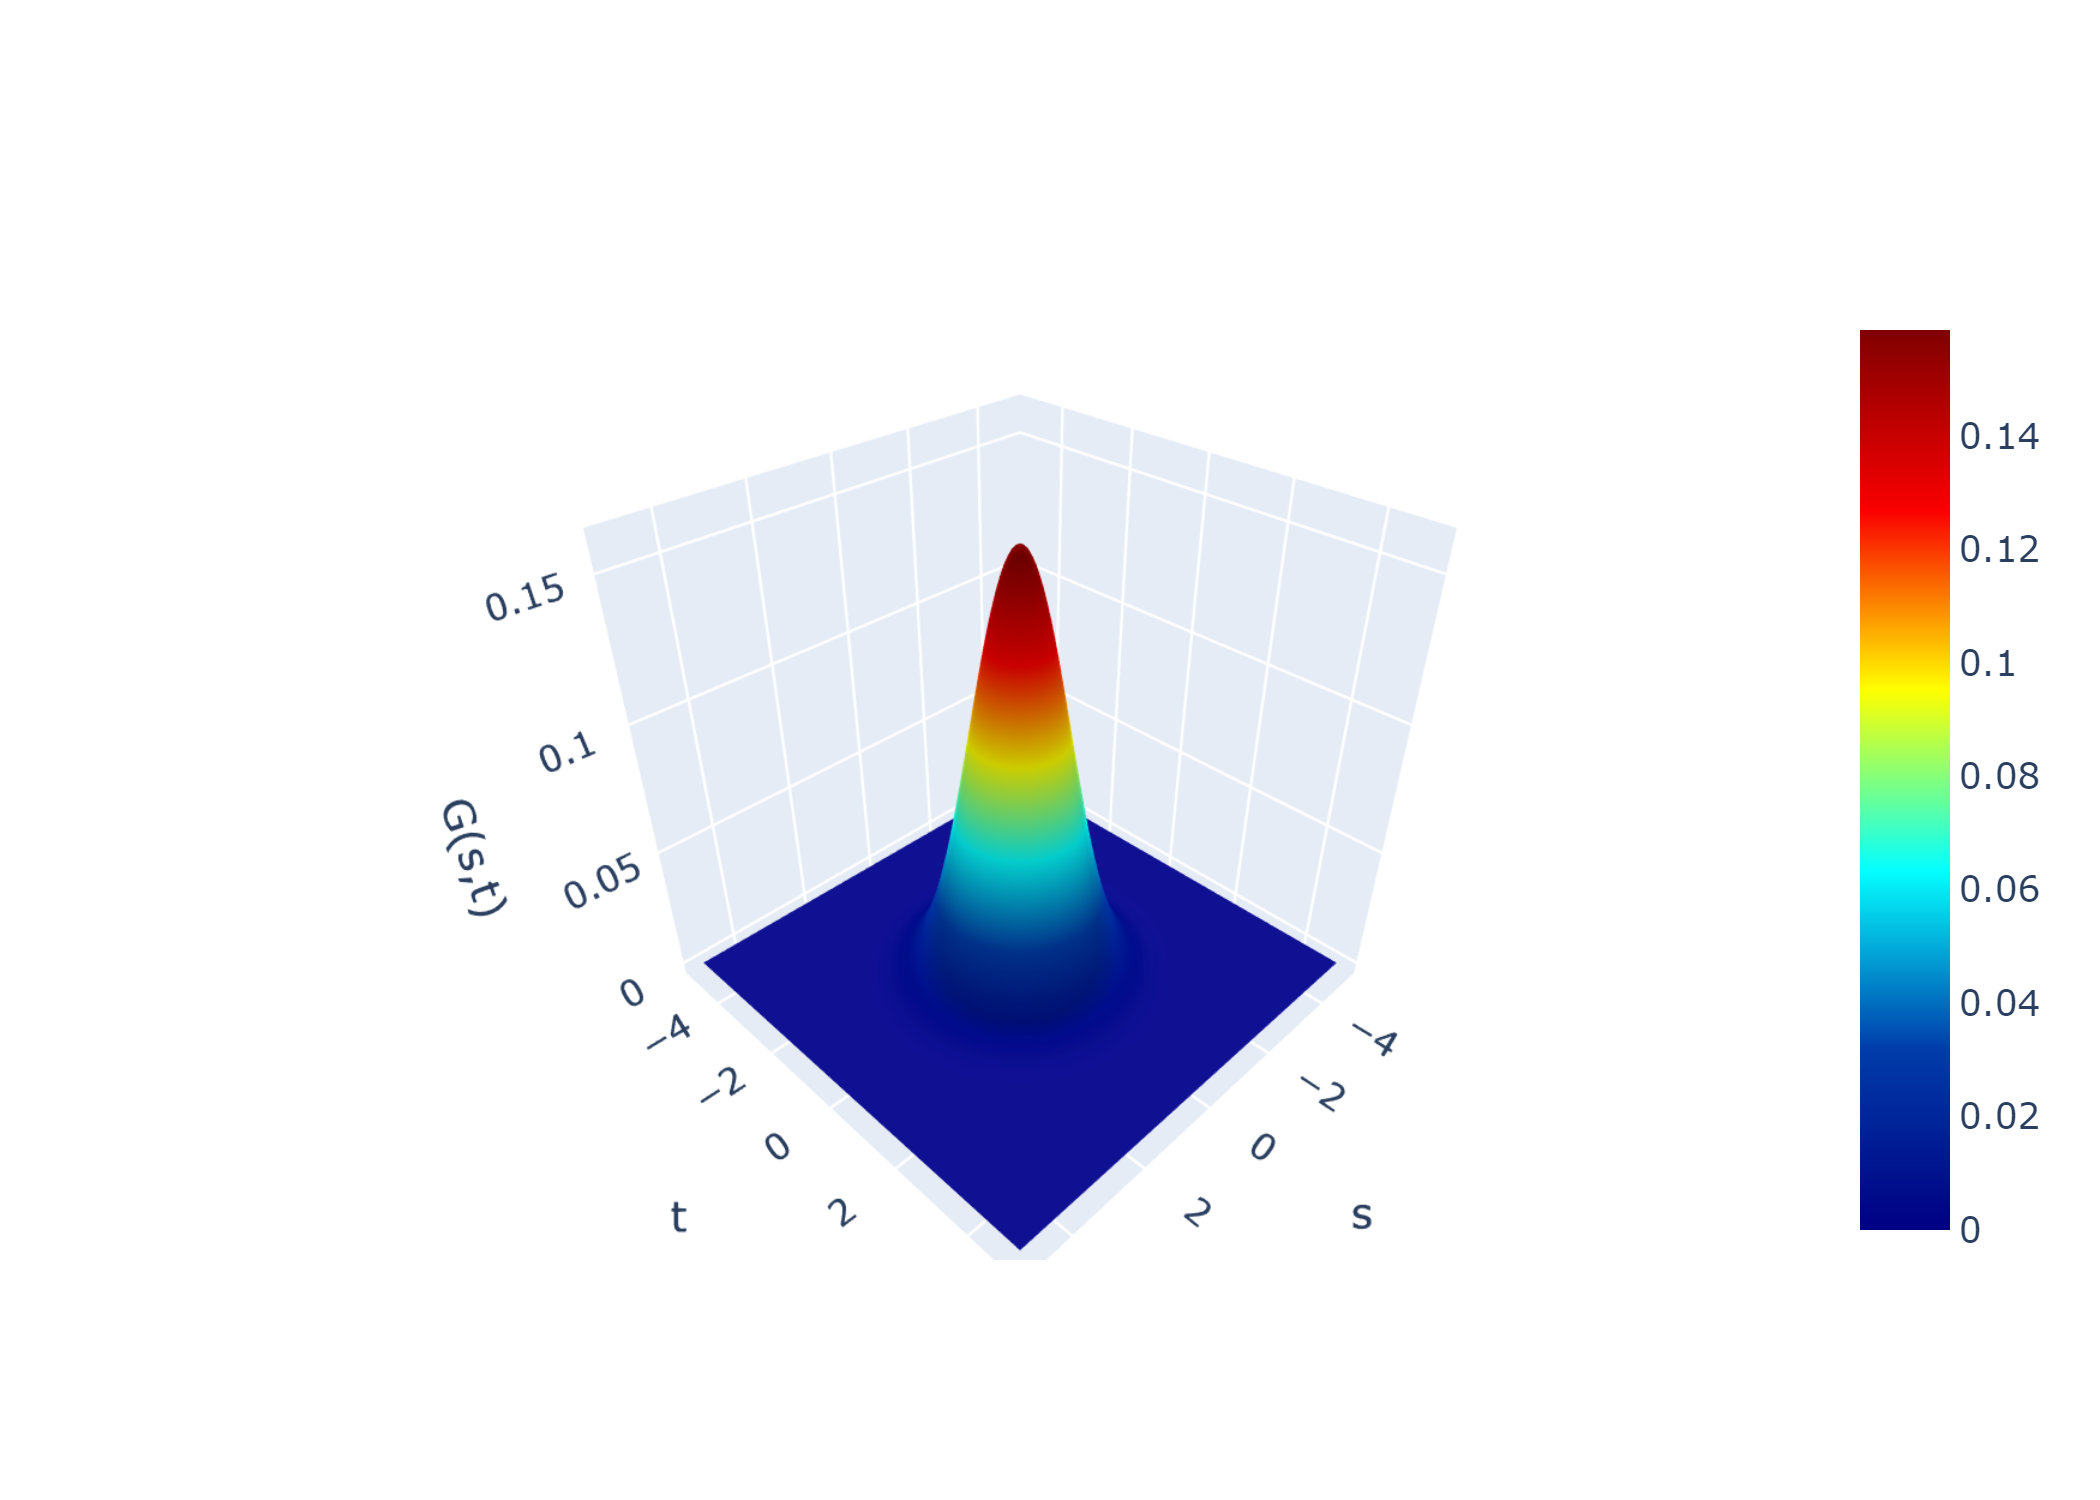
\includegraphics[width=.65\linewidth]{images/Development/chap3/gaussian_3d_plot.png}
\caption{Gaussian distribution.}
\label{fig:gaussian3d}
\end{figure}

A seleção apropriada da dimensão do kernel gaussiano é um aspecto essencial no processamento de imagens. Frequentemente, adota-se um kernel cujo tamanho não exceda $6\sigma$, uma vez que os valores situados além de $3\sigma$ do centro tornam-se praticamente irrelevantes ao resultado final. Tal fenômeno decorre do fato de que a função gaussiana apresenta valores bastante reduzidos a uma distância superior a $3\sigma$ em relação ao seu centro, conferindo-lhes uma importância baixa para a filtragem. A opção por um kernel de dimensões adequadas é fundamental para assegurar um equilíbrio ótimo entre a eficiência computacional e a qualidade do processo de filtragem. A título de exemplo, a Figura \ref{fig:gaussian-example} ilustra a utilização de um kernel gaussiano que obedece a essas características, exemplificando a aplicação prática desses conceitos e enfatizando a relevância de se optar pela dimensão correta do kernel a fim de obter resultados satisfatórios no processamento de imagens \cite{gonzalez_rafael_c_digital_2018}.

\begin{figure}[h!]
\centering
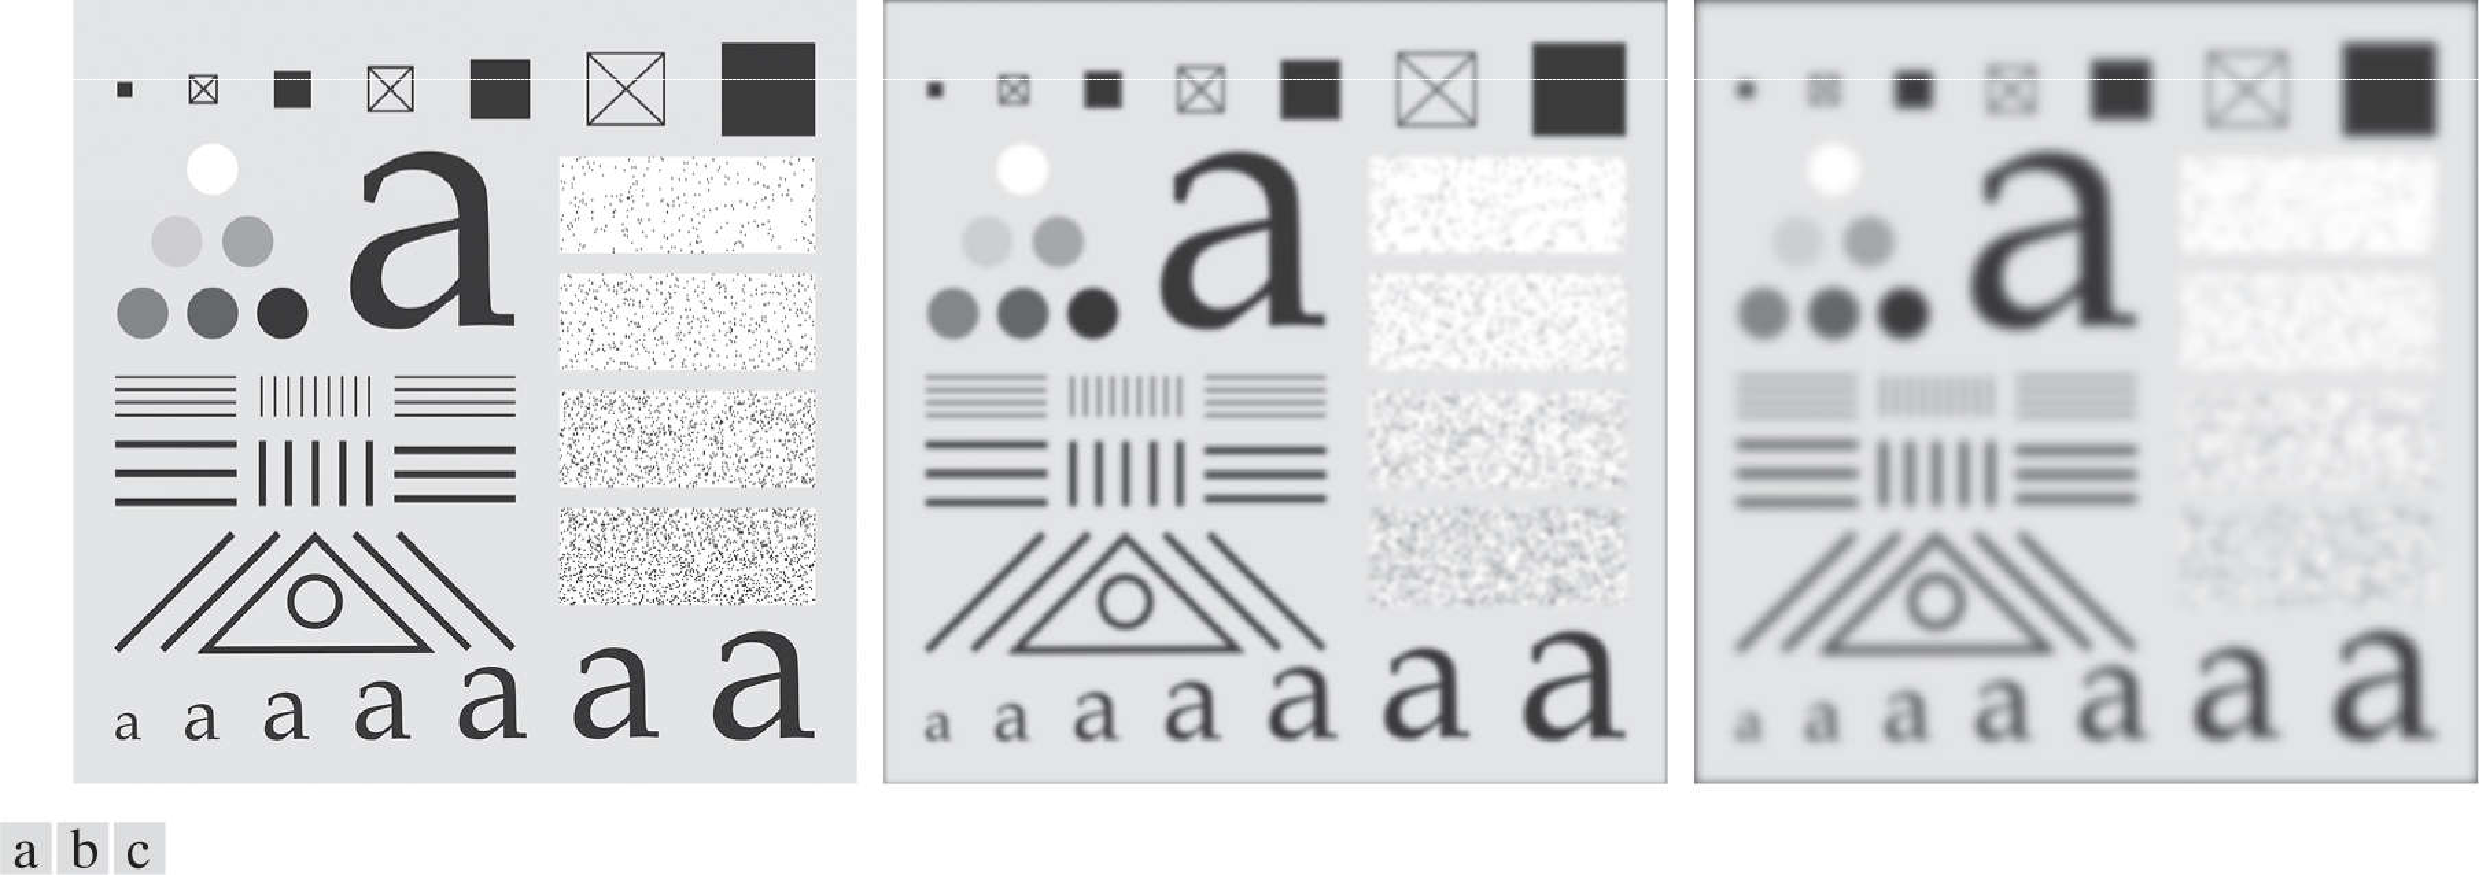
\includegraphics[width=.85\linewidth]{images/Development/chap3/gaussian_example.png}
\caption{(a) A test pattern of size $1024 \times 1024$. (b)  Result of lowpass filtering the pattern with a Gaussian kernel of size $21 \times 21$ with standard deviations  $ \sigma = 3.5 $. (c) Result of using a kernel of size $43 \times 43 $ with  $\sigma = 7 $. We
used in all cases $K = 1$. Source \cite{gonzalez_rafael_c_digital_2018}.}
\label{fig:gaussian-example}
\end{figure}


\subsection{Canny Edge Detection}\label{subsection:Canny-edge-detection}




\section{Embedded System}\label{embeddedSystem}

Exploring the definition and overview of what an embedded system is, as approached by \cite{PECKOL:2008}, it is a combination of hardware and, software parts, as well as other components responsible for running specific tasks. The large amount of applications that make use of embedded systems are intended to work alongside with the physical world, sensing various analog or digital signals while controlling, manipulating, or even responding to others. In order to deal with all the information provided by the signals from the outside and send the data back, the Central Processing Unit (CPU) coordinates the activities of the system, performing communication, computation and data manipulation. 

Commonly, an embedded system consist of a microcontroller programmed to do a specific job. Differently than the microprocessor, as defined by \cite{NISOLOSI:2009}, the microcontroller corresponds to a microprocessor and its typical peripherals, however, now they are all integrated into a single unit. The rich collection of peripherals Input/Output (I/O) into a single integrated circuit, e,g., timers, analog-to-digital converters, digital-to-analog converters, digital I/O, serial or parallel communications channels, etc, it shows the great importance for embedded applications in which low cost is a significant matter \cite{PECKOL:2008}.

In this work, the microcontroller is responsible for receiving the readings from the ultrasonic sensor, manipulating and controlling the information in an orderly manner and send the information to a database (Section~\ref{database}). The Figure~\ref{fig:simpleModelOfTheDataProcess} demonstrates a simple model of the data process and the microcontroller role.

\begin{figure}[h!]
    \centering
    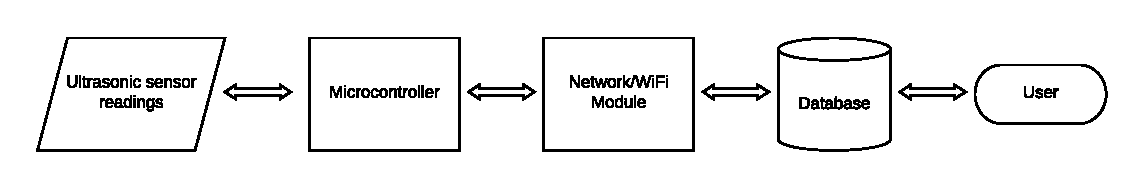
\includegraphics[width=.65\linewidth]{images/study_of_tools/embedded_system/simple_model.pdf}
    \caption{Simple model of the data process.}
    \label{fig:simpleModelOfTheDataProcess}
\end{figure}

In order to store data in a database, the microcontroller makes use of a network module capable to transfer data to a server. So, it is the communication model that makes it possible to interact with other systems \cite{KURNIAWAN:2019}. For that, the ESP32 represents a series of low-cost microcontroller with an integrated network module which is widely used for \gls{IoT} projects and it is used as the microcontroller for the development of this work.


\section{Database Systems}\label{database}

Database systems play a critical role in almost all areas where computers are being used \cite{ELMASRI:2015}. Understanding how someone or some computer program interact with the database are important in order to see how the data can be stored and accessed. There are the traditional database applications whereby the information to be stored and accessed may be either textual and numerical and, there are the noSQL systems (also referred as big data storage systems) by which is mostly used to manage data for social media applications.

As defined by \cite{ELMASRI:2015}, a database is a collection of related data that can be recorded and have implicit meaning. Therefore, the database needs to have some source from which the data is derived in which represents some aspect from the real world. The database can be of any size and complexity and can be managed by the \gls{DBMS}, which is a \textit{general-purpose software system} that is designed to define, manipulate, retrieve and manage data, sharing databases among users and applications. Besides the stored information, defining a database involves specifying data types, structures and constraints of the data to be stored in database, commonly know as database-catalog or meta-data. The manipulation of database comprise functions such as querying the database to retrieve a specific data, update the database and generate reports from the data. Also, the database is shared among users and applications. The Figure~\ref{fig:databaseArchitecture} illustrates a simple database system environment, in which the database and the \gls{DBMS} software build the database system. 

\begin{figure}[h!]
    \centering
    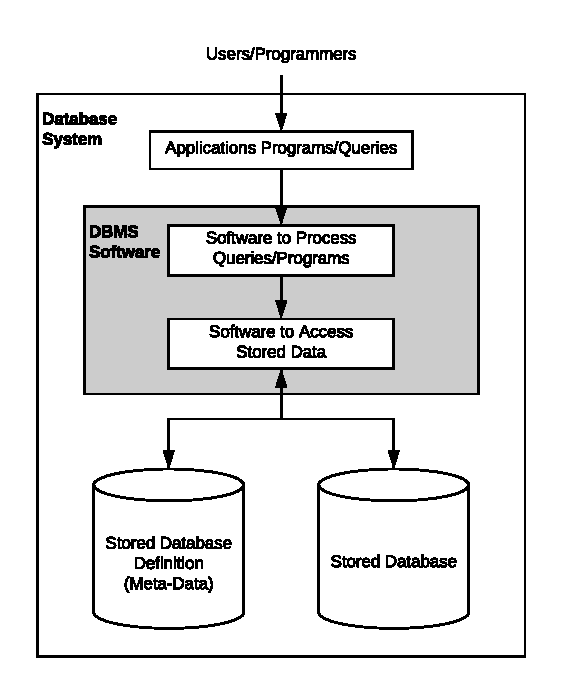
\includegraphics[scale=0.95]{images/study_of_tools/database/SimpleDatabaseArchitecture.pdf}
    \caption{Simple database architecture. Image from \cite{ELMASRI:2015}.}
    \label{fig:databaseArchitecture}
\end{figure}

In a complexity database, typically it can have many types of users which may require different perspectives of the database and must allow multiple users to access the database at the same time. Furthermore, the database needs to have the responsible for design, use and administer a database, and the ones whose are responsible for the development and operation of the \gls{DBMS} \textit{software and system.} Although they are instrumental in making the database available, these workers do not use the contents of the database for their own purpose.


\subsection{Database System Architecture}

The architecture of the \gls{DBMS} packages are based on the client-server system, by which it may be either centralized or distributed across thousands of computers that manage the data stores. In a basic client-server architecture, the client module is designed to run on a user workstation, Personal Computer (PC) or even on mobile devices through application programs and user interfaces (mostly as Graphical User Interface (GUI)) for (PC)s. On the other hand, the server module is responsible for the data storage, access, search and other functions.

The \gls{DBMS} needs an interface with communications software, whose function is to enable the clients to connect via wireless network, Local Area Network (LAN)s and others types of computers networks, to have the access to the database remotely. The Figure~\ref{fig:2tierClientServer} shows the client/server architecture at logic level, the client in this framework is viewed as an user machine with user interface capabilities and local processing, so when the client requires a database access, it connects to a server that provides the request, instead of processing it locally. Already for the server side, it is considered the system which contains both the hardware and software, and is responsible for affording services to the client machines such as printing, archiving or accessing the database. 

\begin{figure}[h!]
    \centering
    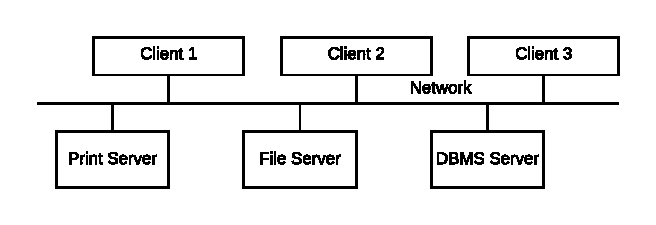
\includegraphics{images/study_of_tools/database/TwoTierClientServer.pdf}
    \caption{Logical two-tier client/server architecture. Adapted from \cite{ELMASRI:2015}.}
    \label{fig:2tierClientServer}
\end{figure}

Basically, for the two-tier architecture, when the \gls{DBMS} is required by the the client side, the program establishes a connection to the \gls{DBMS} (server side), and they can communicate with each other through \gls{API}, provided by Open Database Connectivity (ODBC). In order for this connection to work, both client and server side needs to have the necessary software installed. 

Adding a intermediate layer between the client and the database server, the system becomes three-tier architecture (see Figure~\ref{fig:3tierClientServer}). The middle term, represented by \textit{Tier 1}, is called application server or Web server and it is now responsible for running application programs and procedures or constraints, which may improve the security by verifying the client's credentials before doing a request to database server. Furthermore, the middle layer may work as a Web server, retrieving query results from the database server and formats them into dynamic Web pages, viewed by the client side through Web browser. 

\begin{figure}[h!]
    \centering
    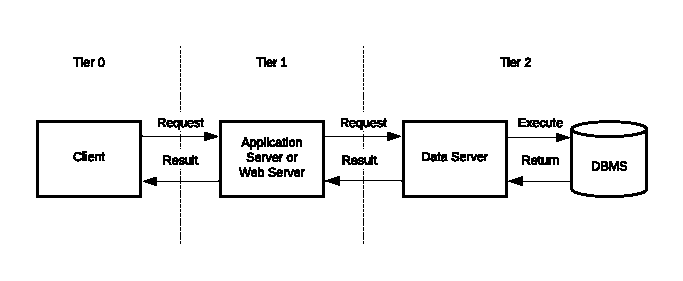
\includegraphics[scale=1.25]{images/study_of_tools/database/ThreeTierClientServer.pdf}
    \caption{Logical three-tier client/server architecture. Adapted from \cite{ELMASRI:2015}.}
    \label{fig:3tierClientServer}
\end{figure}

When using a \gls{RDBMS}, which is a type of \gls{DBMS}, the set of data is stored in table and represents a collection of related data organized in row, column and cells. The interaction with this type of database can be done by typing directly \gls{SQL} commands into a monitor for execution by the database system. However, mostly of databases interactions are executed through application programs, commonly known as database applications, and they are normally developed in a general-purpose programming language such as Java, C/C++/C\#, or even in some other programming languages. Recently, some script languages, e.g, \gls{PHP}, JavaScript and Python, have become widely used for programming of database access within Web applications. In this work, all \gls{API}s were written in \gls{PHP} and it will be approached in the Section~\ref{section:database}.


\subsection{Sequence of Interaction in Database Programming}\label{sequenceOfInteraction}

In order to have an understanding about the sequence of interaction in database programming, a common sequence is adopted and it can be divided in three steps.

First, when the client requires an access to a particular database, the application program or Web server is the one responsible for enabling this interaction between them. Regularly, the client request is specify by the Internet address \gls{URL} of the machine where the database server is located, and uses a \gls{HTTP} with specific know \gls{HTTP} methods, to indicate the desired action to be performed, e.g., GET, POST, HEAD, DELETE, etc. After the request is done, the program must first \textit{establish} or \textit{open} a connection to the database server and provide a login account name and password to have the access to the database server (see Figure~\ref{fig:httpRequest}). 

\begin{figure}[h!]
    \centering
    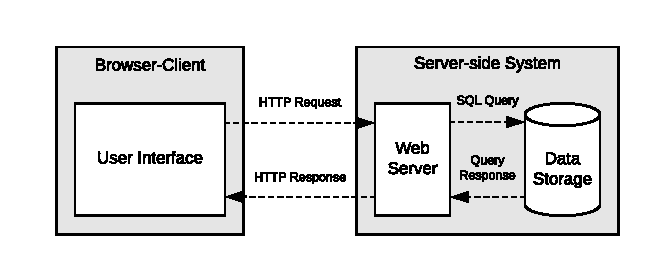
\includegraphics[scale=1]{images/study_of_tools/database/HTTPrequest.pdf}
    \caption{Basic diagram of HTTP request/response. Adapted from \cite{ELMASRI:2015}.}
    \label{fig:httpRequest}
\end{figure}

As soon the connection is \textit{established}, the program can interact with the database server by submitting queries, updates and other database commands. As a result, the server returns a \gls{HTTP} response to the client in which it may contains information about the request as desired.

Lastly, when the program execute all the necessary functions and no longer needs access to a database server, it must \textit{terminate} or \textit{close} the connection with the database.


\section{Web Development}\label{webDevelopment}

This section provides an overview of the languages used for the development of a basic Web site, either for client-side and server-side model, commonly know as front end and back end, respectively. These terms are used to refer the difference between the presentation layer viewed by the client and the data access layer. The concepts of developing a Web page involve simple static pages of plain text to complex based-web applications with dynamic content. Therefore, different languages approaches can be taken according to the model that best suits the application.

\subsection{Server-side Programming using PHP}

The \gls{PHP} is a language that runs directly on the server and it is used as a pipeline that collects client user input through forms, formulate database queries and submits them to the database, creating dynamic \gls{HTML} Web pages. Although there are other server-side languages such as Java Servlets, Java Server Pages (JSP) and JavaScript, which use a type of JavaScript called Node.js for server-side work, all the \gls{API}s were written in \gls{PHP} and this overview is only going to cover the \gls{PHP} script language. 

The method of \gls{PHP} to connect with any \gls{RDBMS}, as introduced by \cite{SQUIER:2004}, it is based on following the steps as approached in the Section~\ref{sequenceOfInteraction}. These steps can be done by using some \gls{PHP} functions such as \textit{mysql\_connect()} and \textit{mysql\_close()}, which allows the application program to interact with the database server.

Once the connection is established, it is possible to retrieve and manipulate data from My\gls{SQL} database. For retrieving data, it can be used \textit{SELECT} statements with \textit{mysql\_query()} and, the returned result identifier is passed into result memory, which can be stored in a variable normally called \textit{\$result}. Already for the manipulation of user records, it is used functions to insert, update and delete records in tables using \textit{INSERT}, \textit{UPDATE} and \textit{DELETE} statements, respectively. These basic functionalities are suitable for enabling the data from the ultrasonic sensor to be stored and manipulated in a MySQL database.


\subsection{Client-side Programming Language}\label{section:clienteSide}

As studied by \cite{FELKE-MORRIS:2019}, the \gls{HTML} is one of the language used to create web pages and it basically consist of sets of directions that tell the browser software how to display and manage a web document. The commonly know name for these directions are called tags and it performs functions such as displaying graphics, formatting text and referencing hyperlinks.

These markup symbols and codes can identify structural elements such as paragraphs, headings and lists such a way that, when the browser interprets the markup code, it will render the page, independently of what type of computer the web page was created. Therefore, any browser running on any operating system will be capable of displaying the web page.

Essentially, there are two sections on a web page and they are separated in head and body. The head section contains information about the title of the web page, the meta tags which describe the documents and references to script and style of the web page. Already for the body section, it includes elements that display directly in the browser window (browser viewpoint). These elements are represented and manipulated by the Document Object Model (DOM), which is the fundamental \gls{API} that treats the \gls{HTML} document as a tree structure, wherein each node represents tags and elements of the document.

The \gls{HTML} is composed by structural elements as show in Figure~\ref{fig:structuralElements}. These elements have been used for many years as they configure structural areas or divisions on a web page. While the \gls{HTML} is responsible for the website structure, the \gls{CSS} is responsible to deal with the text, color and page layout. It provides functionalities by providing typographic styles and space instructions to printed media. As can be noticed in Figure~\ref{fig:cssStructured}, the typographic and page layout may be better controlled, also, the style is separate from the web page structure, allowing the configuration to be stored, all of these features make the document smaller and the site maintenance easier.

\begin{figure}[htpb!]
    \centering
    \subfigure[Structural elements of a web page.]{
        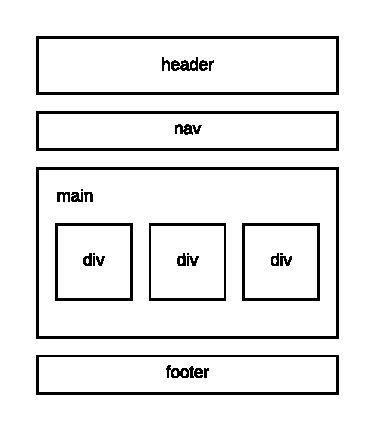
\includegraphics[scale=0.85]{images/study_of_tools/web_development/structuralElements.pdf}
        \label{fig:structuralElements}
    }
    \subfigure[The power of a single CSS file.]{
        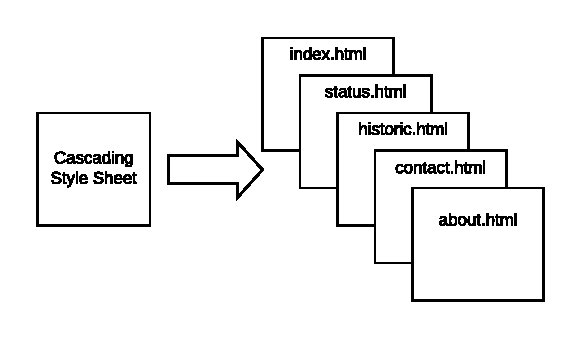
\includegraphics[scale=0.95]{images/study_of_tools/web_development/cssStructure.pdf}
        \label{fig:cssStructured}
    }
    \caption{HTML and CSS structure. Adapted from\cite{FELKE-MORRIS:2019}.}
    \label{fig:html&css}
\end{figure}

Albeit the \gls{HTML}/\gls{CSS} can work very well together, in order to add interactivity into web page then just simple static pages of plain text, it is necessary embedding the JavaScript in \gls{HTML}, as approached by \cite{FLANAGAN:2011}. The use of JavaScript in Web Documents can define the \textit{behavior} of document elements by invoking an appropriate \textit{event handler} function to respond to each event accordingly, whereby the properties of these event handler have names that begins with the word "on", e.g., \textit{onload, onclick}. The combination of scriptable content, presentation and behavior is called \gls{DHTML}. 

The best know of the features brought by \gls{DHTML} is the XMLHttpRequest object, which enables networking through scripted \gls{HTTP} requests \cite{FLANAGAN:2011}. This is a part of the Web 2.0 movement, which makes the transition of the Web from isolated static websites to a platform, with interfaces that can obtain new information from the server without a page load. This is called \gls{AJAX} and it is a web development technique that pushes more of the processing on the client by using JavaScript and Extensible Markup Language (XML) and sometimes, behind-the-scene, asynchronous requests to the server to refresh a portion of the browser display, instead of loading the entire web page \cite{FELKE-MORRIS:2019}.

Another important point, when an \gls{API} is requested, by an \gls{AJAX} method, to push elements data from the server, the server's response takes the form of \gls{JSON} string, which is a lightweight data-interchange format used for data exchange between the server and the client. Therefore, in order to retrieve the useful information received back from the web server, the \gls{JSON} string is parsed using JSON.parse() method, which is responsible for parsing the \gls{JSON} string and constructing the JavaScript value or object described by the string. However, as the JSON.parse() method is a JavaScript's standard built-in \gls{JSON} object method, it means that it may not be supported by some browsers (in case of the old ones). A solution for that is to use jQuery, which is a JavaScript library that is written on top of JavaScript, i.e., it makes use of JSON.parse() method internally. This library is browser independent, so if the JSON.parse() is not available, the jQuery can be responsible for parsing the JSON string.